\documentclass[a4paper,12pt]{article}

\usepackage[utf8]{inputenc}
\usepackage[T1]{fontenc}
\usepackage[czech]{babel}
\usepackage{amsmath}
\usepackage{amsfonts}
\usepackage{amssymb}
\usepackage{graphicx}
\usepackage{hyperref}
\usepackage{float}
\usepackage{hyperref}

\usepackage[a4paper]{geometry}
\geometry{verbose,tmargin=2.5cm,bmargin=2cm,lmargin=2cm,rmargin=2cm}
\usepackage{fancyhdr}
\pagestyle{fancy}

% nastaven� pisma a �e�tiny
\usepackage{lmodern}
\usepackage[T1]{fontenc}
% v�cesloupcov� tabulky
\usepackage{multirow}

% vno�en� popisky obr�zk�
\usepackage{subcaption}

% automatick� konverze EPS 
\usepackage{graphicx} 
\usepackage{epstopdf}

% odkazy a z�lo�ky


% Pozn�mky p�i p�ekladu
\usepackage{xkeyval}	% Inline todonotes
\usepackage[textsize = footnotesize]{todonotes}
\presetkeys{todonotes}{inline}{}


\title{Řešení úkolu pro TurtleBot s detekcí objektů a SLAM}
\author{Michal Bouda, Erik Doležal, Ondřej Váňa}
\date{\today}

\begin{document}

\maketitle

\tableofcontents

\section{Zadání}
Úkolem práce je napsat řešení úkolu, kde má Roomba TurtleBot kopnout míč do branky označené modrými pilíři.
Rozložení problému je vidět na obrázku \eqref{fig:map}.
\begin{figure}[H]
\centering
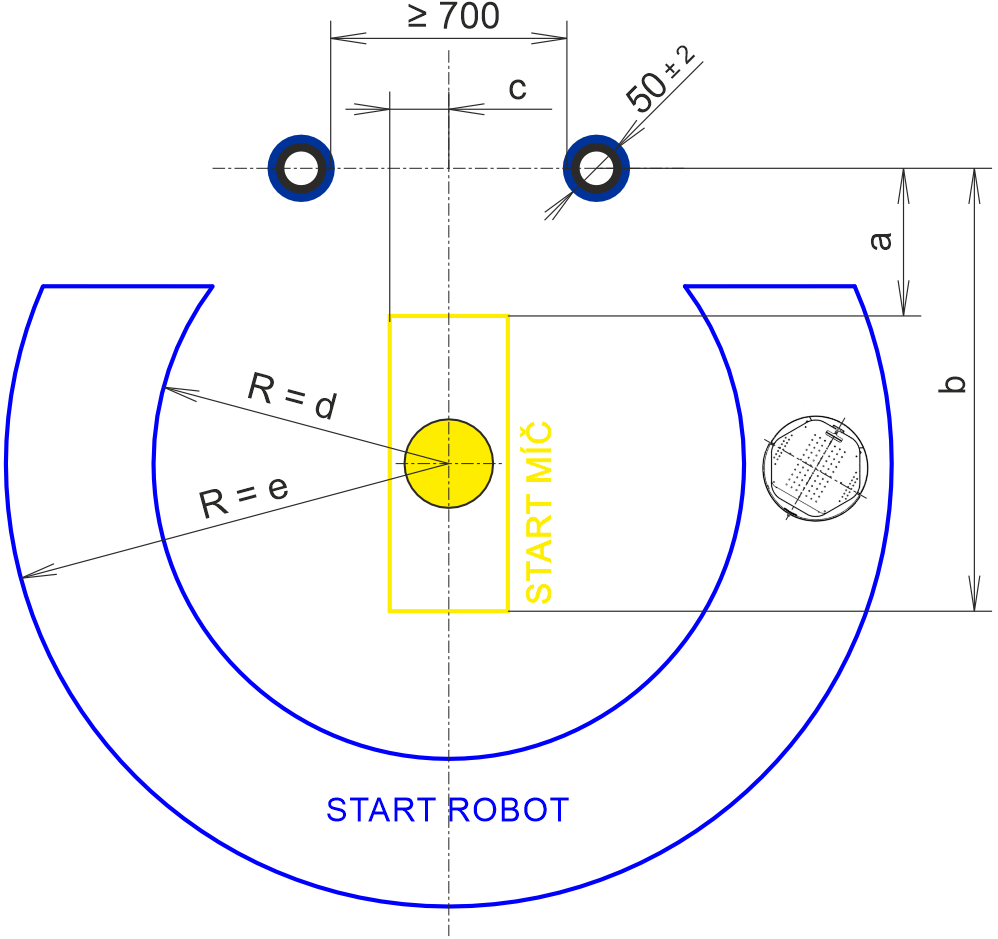
\includegraphics[width=0.4\textwidth]{pictures/map.png}
\caption{Rozložení objektů v prostoru (ze zedání)}
\label{fig:map}	
\end{figure}

\subsection{Úloha 2}
Robot má za úkol najít míč a ten kopnout mezi modré pilíře, které jsou od sebe vzdálené minimálně $700$ mm. Robot musí zastavit $20$ cm před brankou. Míč je vzdálen od osy branky maximálně $c = 150$ mm.
Míč se bude nacházet v minimální vzdálenosti $a = 500$ mm od brány a bude nejdále $b = 1,5$ m. TurtleBot bude na začátku umístěn od středu míče ve vzdálenosti $d = 0,7$ m až $e = 2,5$ m.
Za bránou může být neomezený počet pilířů.

\subsection{Úloha 3}
Od Úlohy 2 se Úloha 3 liší tím, že míč může být vzdálen od osy branky $c = 300$ mm. Vzdálenost míče od branky může být až $b = 2$ m.
Největším rozdílem je možnost výskutu až dvou překážek před čarou. Ty jsou umístěny tak, že pokaždé existuje cesta od míe k brance o minimální šířce $600$ mm.

\section{Řešení}
Naše řešení jsme rozdělili na tři hlavní části. První část je zpracování obrazu, druhá část je SLAM a třetí část je plánování a pohyb robota. Tyto části běží v hlavní smyčce programu. Naše řešení je dimenzováno pro řešení třetí úlohy. Z nedostataku času pro ošetření všech možných přídapů, jsme se ale rozhodli řešit druhou úlohu. 
Při řešení problému bylo využíváno nástroje GitHub Copilot pro jednoduché úkony pro zrychlení práce. 
\subsection{Zpracování obrazu}
Detekci objektů děláme pomocí konvoluční neuronové sítě \href{https://docs.ultralytics.com/models/}{YOLO} (You Only Look Once), kterou poté konvertujeme do \href{https://onnx.ai/}{ONNX}. Důvodem k použití CNN bylo, aby náše řešení dobře zvládalo změny v osvětlení a jiné rušivé vstupy jako například špinavý žlutý míč. Segementace obrazu pomocí barev, by mohla být v tomto ohledu nespolehlivá. Jako vstup používáme obraz z Intel RealSense D435 kamery.
\subsubsection{Trénování CNN}
YOLO model jsme museli nejdříve natrénovat na rozponávání pilířů a míče. Učinili jsme tak na více než 670 obrázcích,
které jsme pořídili pomocí kamery na robotovi. Dalších 120 jsme použili pro validaci. Obrázky jsme ručně anotovali pomocí programu \href{https://labelstud.io/}{Label Studio}. Jak vypadá anotace je vidět v obrázku \eqref{fig:label_studio}.
\begin{figure}[H]
    \centering
    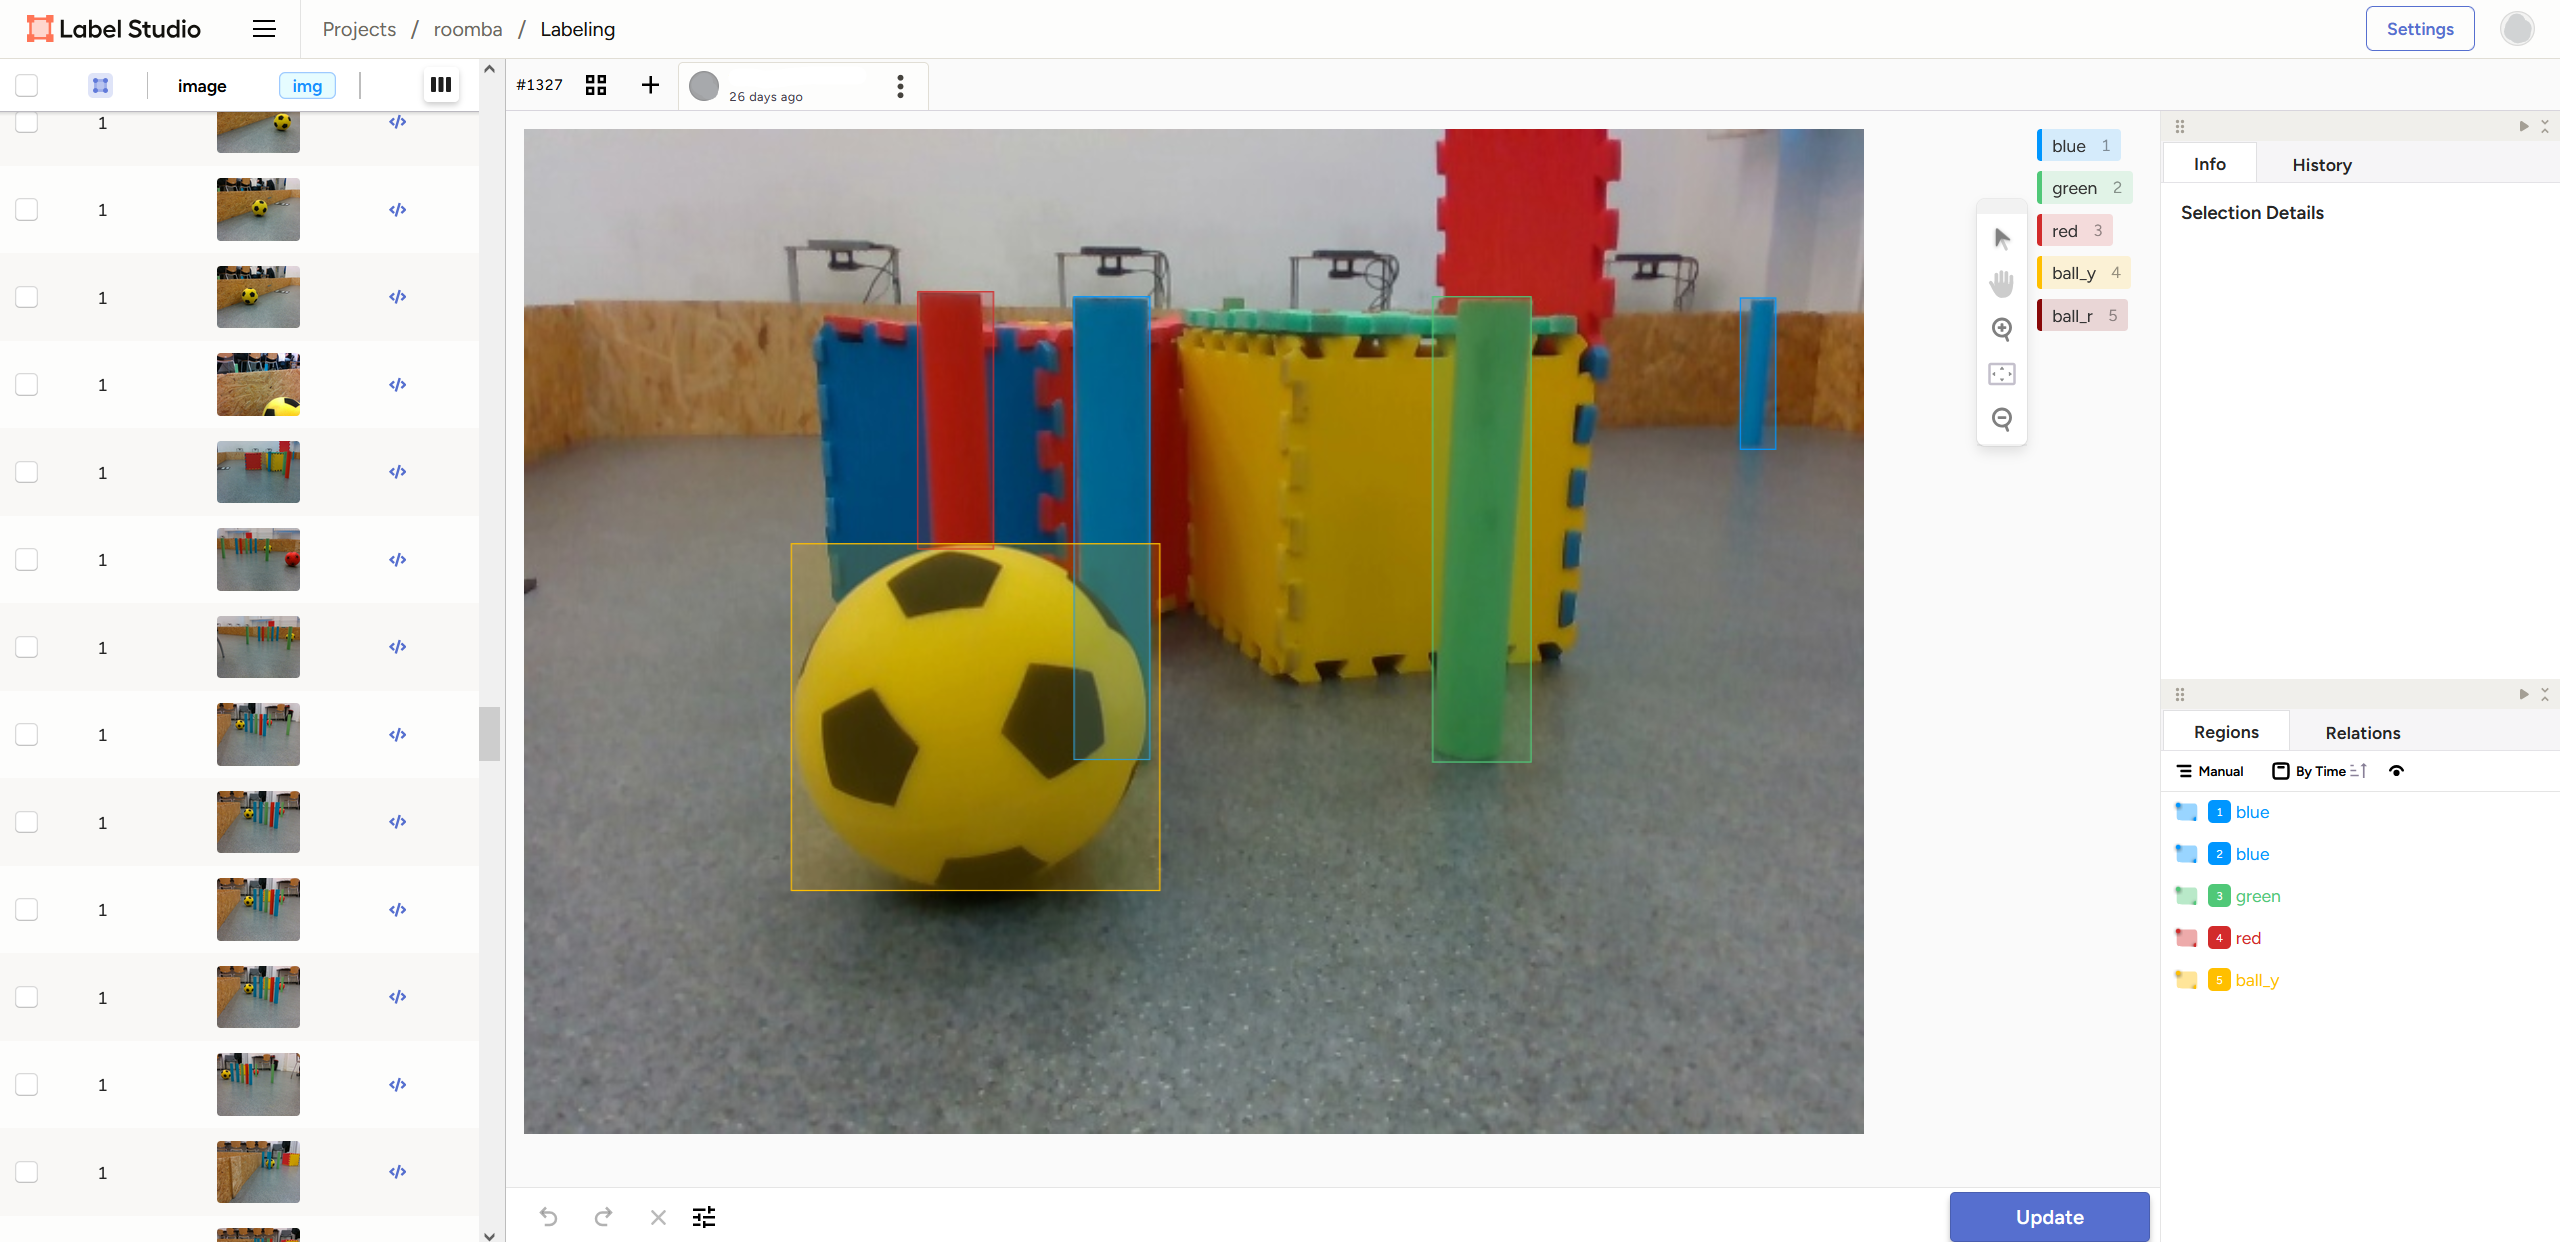
\includegraphics[width=0.8\textwidth]{pictures/label_studio.png}
    \caption{Anotování v Label Studiu}
    \label{fig:label_studio}	
\end{figure}
Pro anotaci jsme použili nastavení \textit{Object Detection with Bounding Boxes}, tedy jsme anotavali pomocí obdelníků. Zvolili jsme možnost bez rotace, všechny obdelníky mají tedy rovnoběžné strany se stranami obrazu. 
Toto představilo problém, který jde vidět v obrázku \eqref{fig:detected_image}. Díky zakřivení obrazu z kamery, obdelníky nesedí přímo na pilíře, což byl lehce vyřešitelný problém \eqref{sec:point_cloud}. Možnost segmentace, myšleno maskou jsme zamítli z různých důvodou, např. pracné anotace. 
Anotovaný data set byl poté vyexportován ve formátu YOLO.
Pomocí Python kódu a knihovny od \href{https://docs.ultralytics.com/}{Ultralitics} jsme natrénovali model. Vyzkoušeli jsme YOLO verze v8 a 11. Ukázalo se, že verze 11 je mnohem přesnější, zvláště při změně osvětlení. 
Protože detekce musí probíhat rychle, zkoušeli jsme modeli 11s a 11n. I když je model 11s přesnější, používáme ho jen výjimečně, protože může způsobit problémy pro SLAM svojí dlouhou časovou náročností. 
I pro model 11n jsme zkoušeli různé rozlišení. Rozlišení 160p a 240p bylo zpracováno dostatečně rychle a s uspokojivími výsledky. Oba modely byly natrénovany na 300 epochách.

\begin{figure}[H]
    \centering
    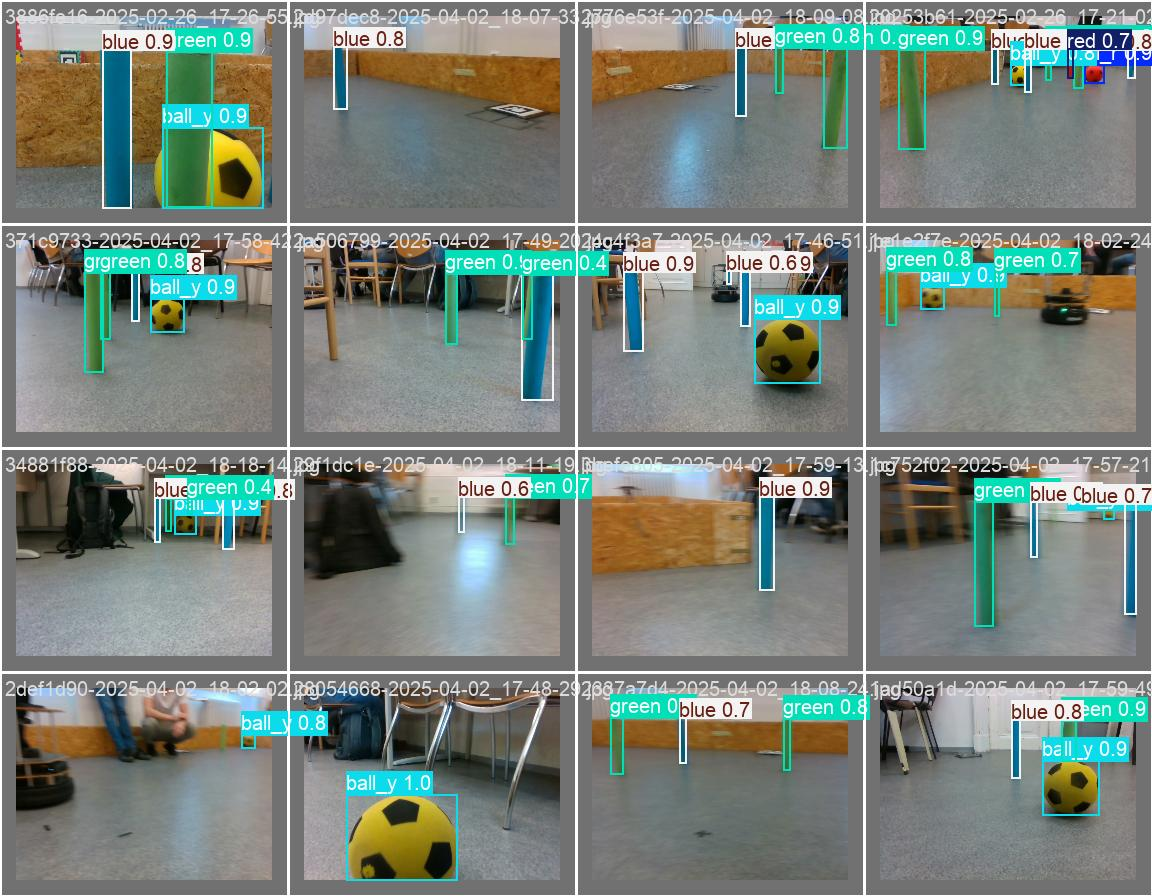
\includegraphics[width=0.7\textwidth]{pictures/rozpoznane.jpg}
    \caption{Rozpoznané objekty pomocí YO
    LO 11n při rozlišení 240p}
    \label{fig:detected_image}
\end{figure}

\begin{figure}[H]
    \centering
    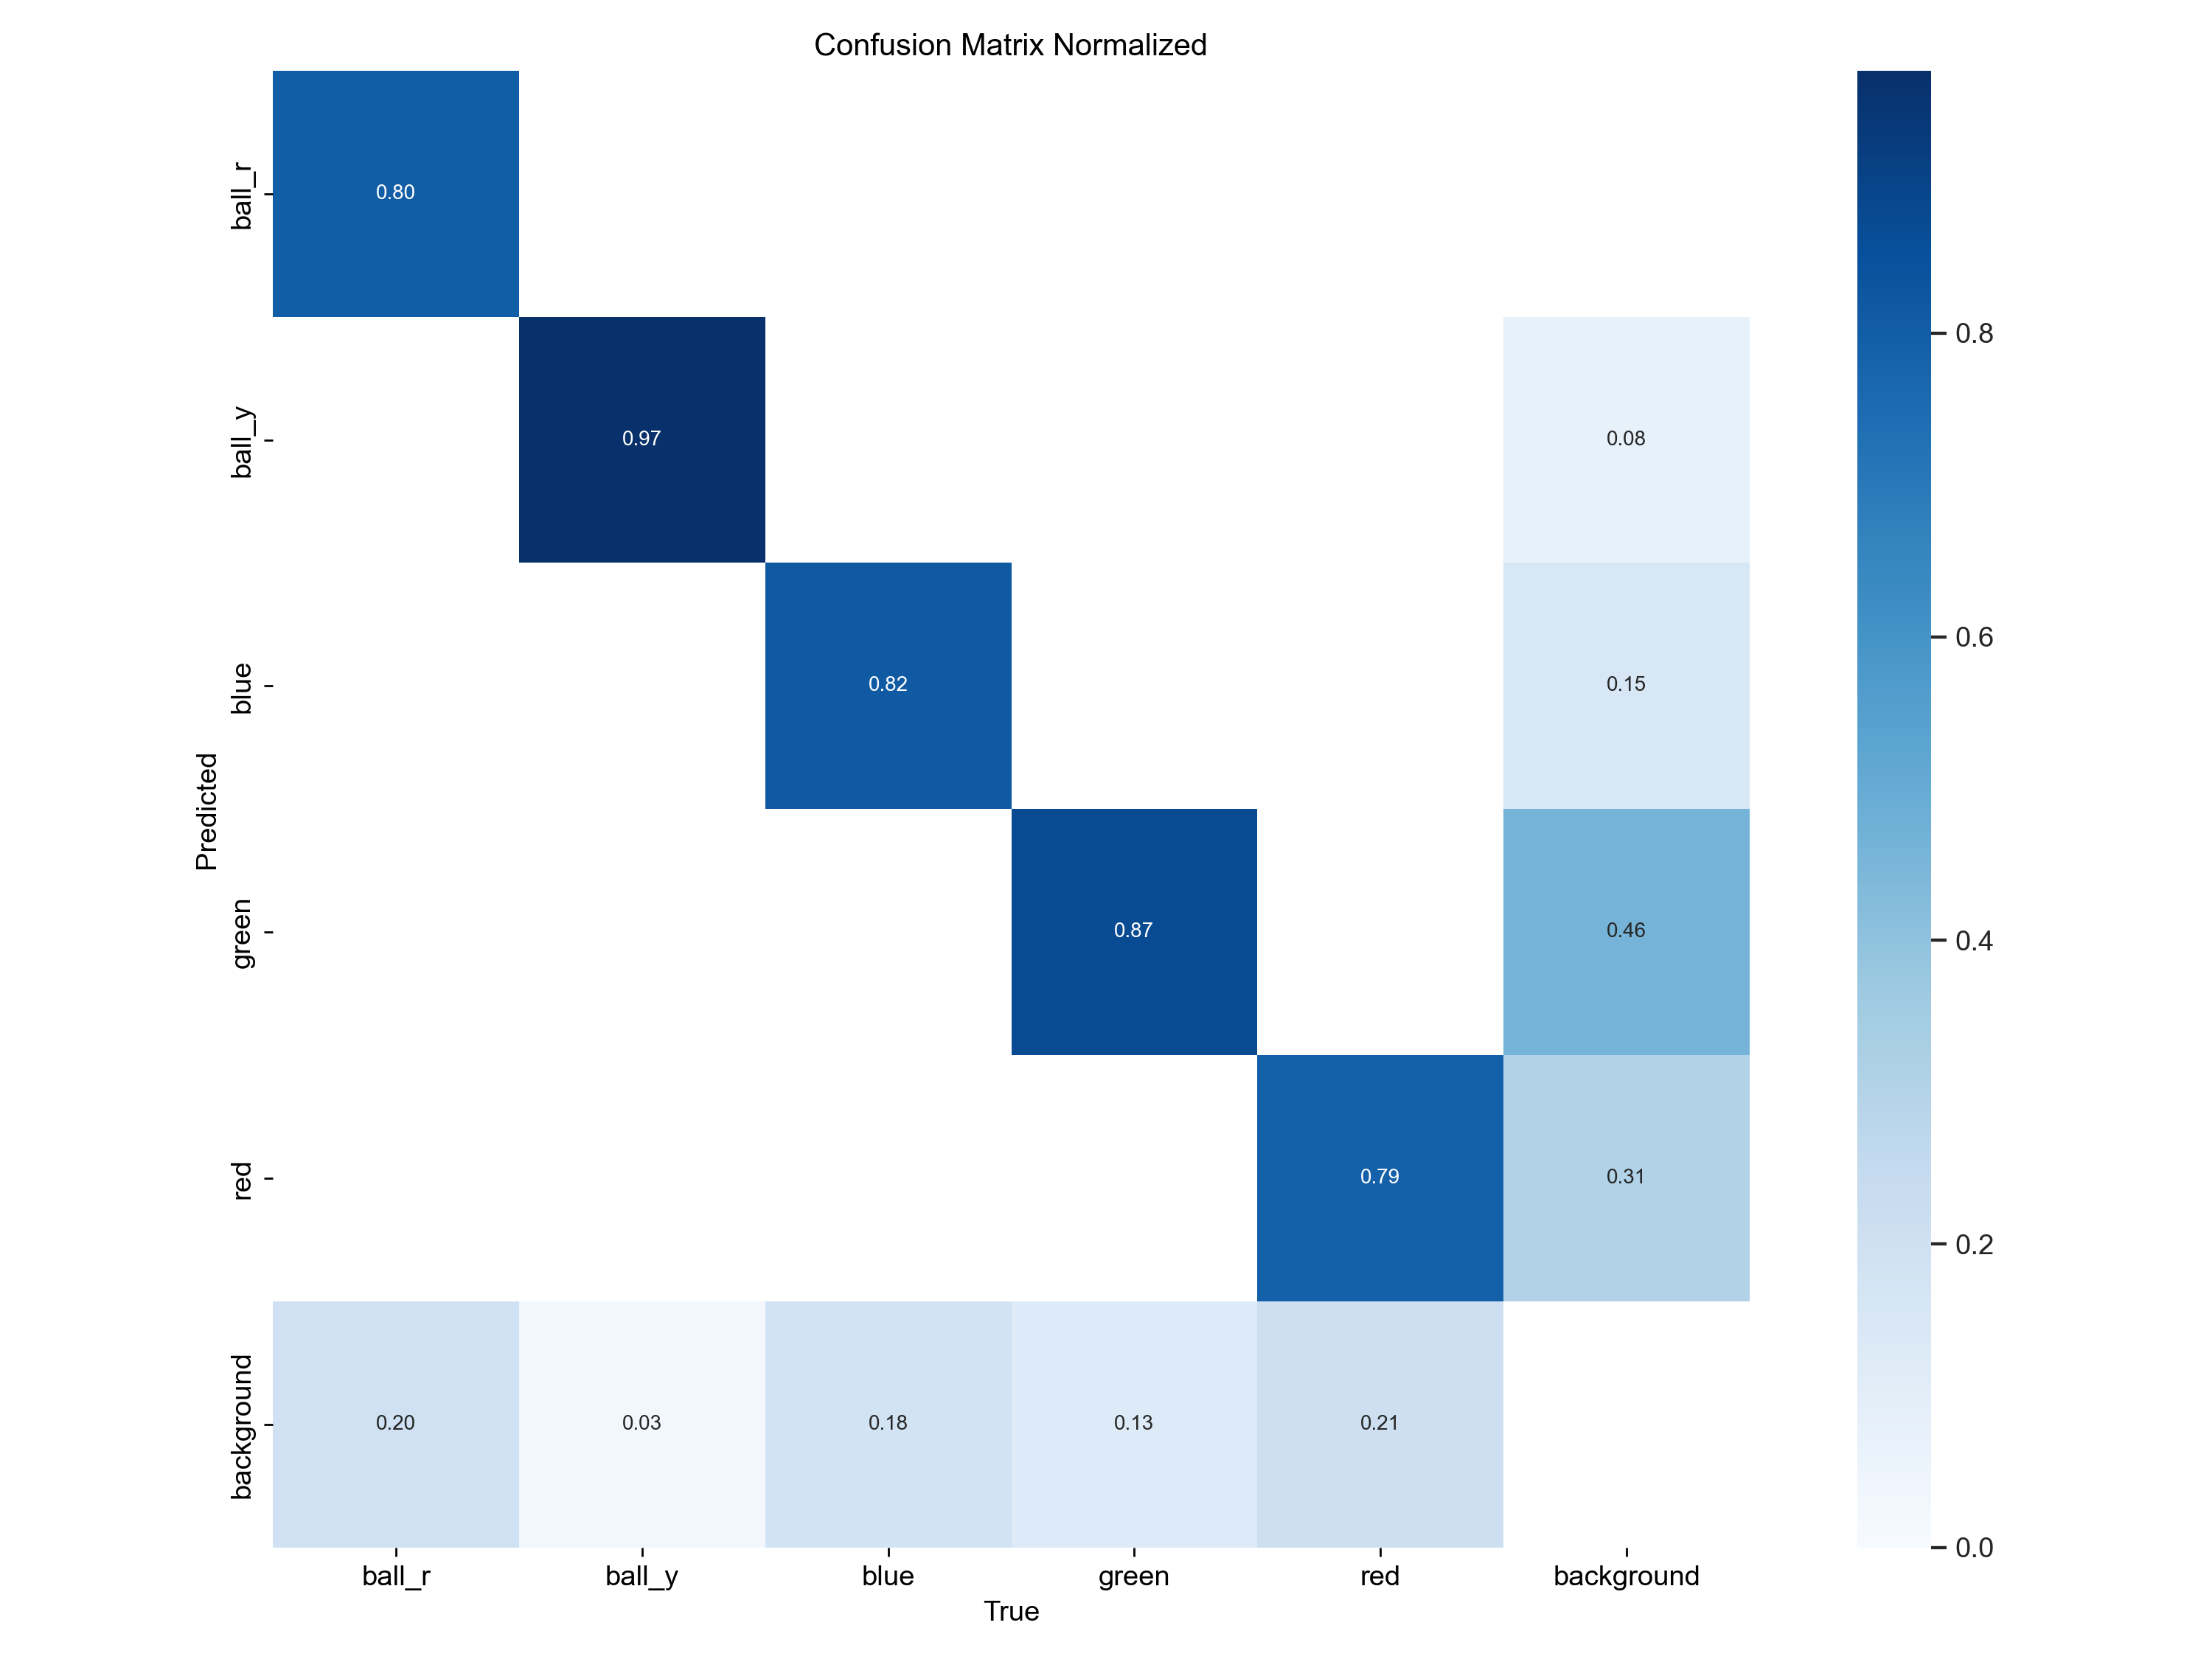
\includegraphics[width=0.8\textwidth]{pictures/v11n_160p.png}
    \caption{Normalizovaná matice záměn pro model 11n 160p}
    \label{fig:confusion_matrix_160p}
\end{figure}

\begin{figure}[H]
    \centering
    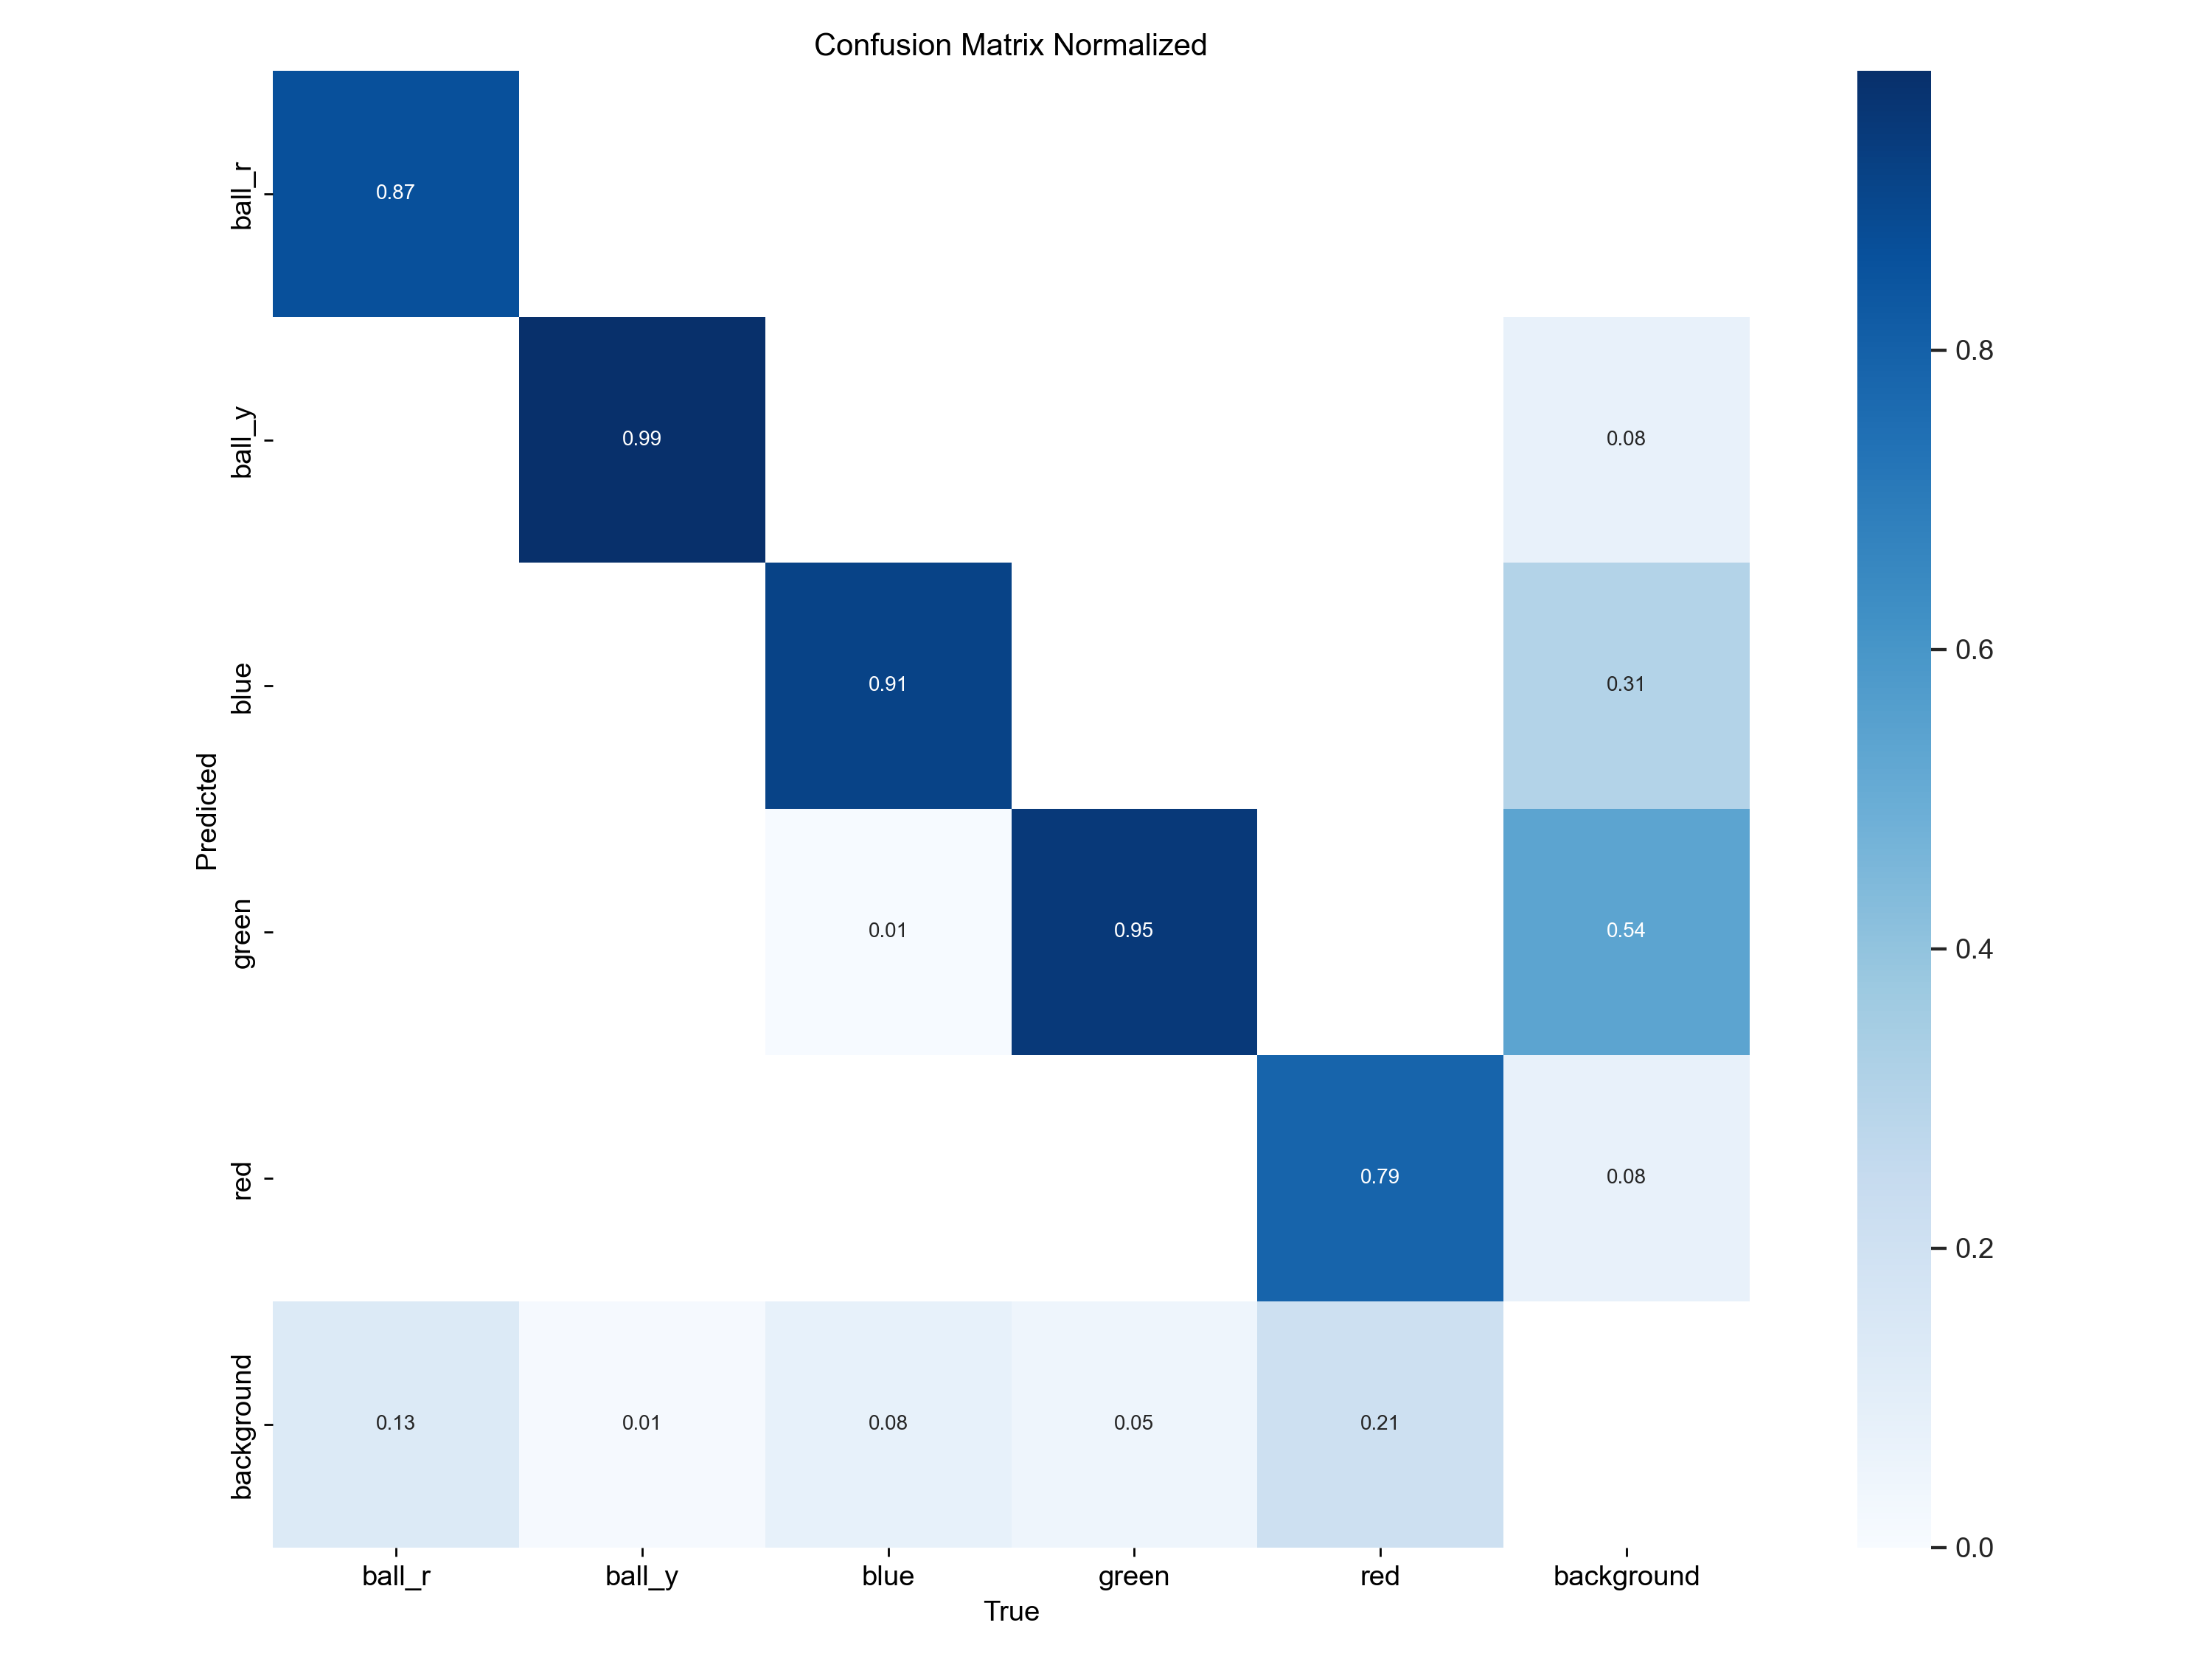
\includegraphics[width=0.8\textwidth]{pictures/v11n_240p.png}
    \caption{Normalizovaná matice záměn pro model 11n 240p}
    \label{fig:confusion_matrix_240p}
\end{figure}

Model 160p (Obrázek \eqref{fig:confusion_matrix_160p}) je v některých podmínkách znatelně horší oproti 240p (Obrázek \eqref{fig:confusion_matrix_240p}) v rozpoznávání modrých pilířů.
To může způsobit velké problémy, protože modré pilíře tvoří branku. Nejčastějším objektem, který byl zaměněn s pozadím, je zelený pilíř, který, když je detekován navíc, minimálně překaží úspěšnému vyřešení problému.
V obrázku \eqref{fig:detected_image} si ještě můžeme všimnout, že model dobře zvládá rozpoznávání objektů, které mají zaměnitelné barvy nebo tvar s objekty, které detekuje.
Model také například rozpoznal míč, když je z části za pilířem, nebo objekty, když jsou ve stínu pod stolem.

\subsubsection{Rozpoznávání obrazu}
K rozpoznávání použiváme buď model YOLO 11n při rozlišení 160p nebo při 240p v závislosti na prostředí a pokud více benefitujeme z rychlejší detekce nebo její přesnosti.
Na robotovi zajišťuje rozpoznávání class \texttt{Camera}. Třída má metodu \texttt{get detections}, která získá obraz z kamery. 
Seznam objektů vracíme pro potřeby SLAM jako numpy array poloha x, poloha y, objekt. Poloha x, y je poloha relativně k robotovi v prostoru.

K detekci nepoužíváme samotnou knihovnu YOLO. Model nejdříve konvertujeme do ONXX (Open Neural Network Exchange). Důvodem pro toto rozhodnutí je dlouhá doba, kdy YOLO knihovna zpracovála obraz. ONNX to zvládá rychleji z části díky tomu, že je optimalizovaná pro spouštění na procesoru.
Používání ONNX ale přineslo spoustu výzev, protože YOLO knihovna řešila spoustu věci za nás. Museli jsme naimplementovat počítaní pravděpodobností detekce pomocí softmax. 
Poté pomocí Non-Maximum Suppression z knihovny TorchVision řešíme odstranění duplicitních detekcí. A samozřejmostí je nepracování s detekcemi, které nedosahují nějaké hranice jistoty.

\subsubsection{Pozice objektů v prostoru}
\label{sec:point_cloud}
Z počátku jsme využívali k určování pozice objektů point cloud, který jsme získali z kamery.
To se ukázalo jako velice časově náročné. Proto jsme se rozhodli, že budeme počítat pozici objektů přímo z hloubkové kamery.
\begin{figure}[H]
    \centering
    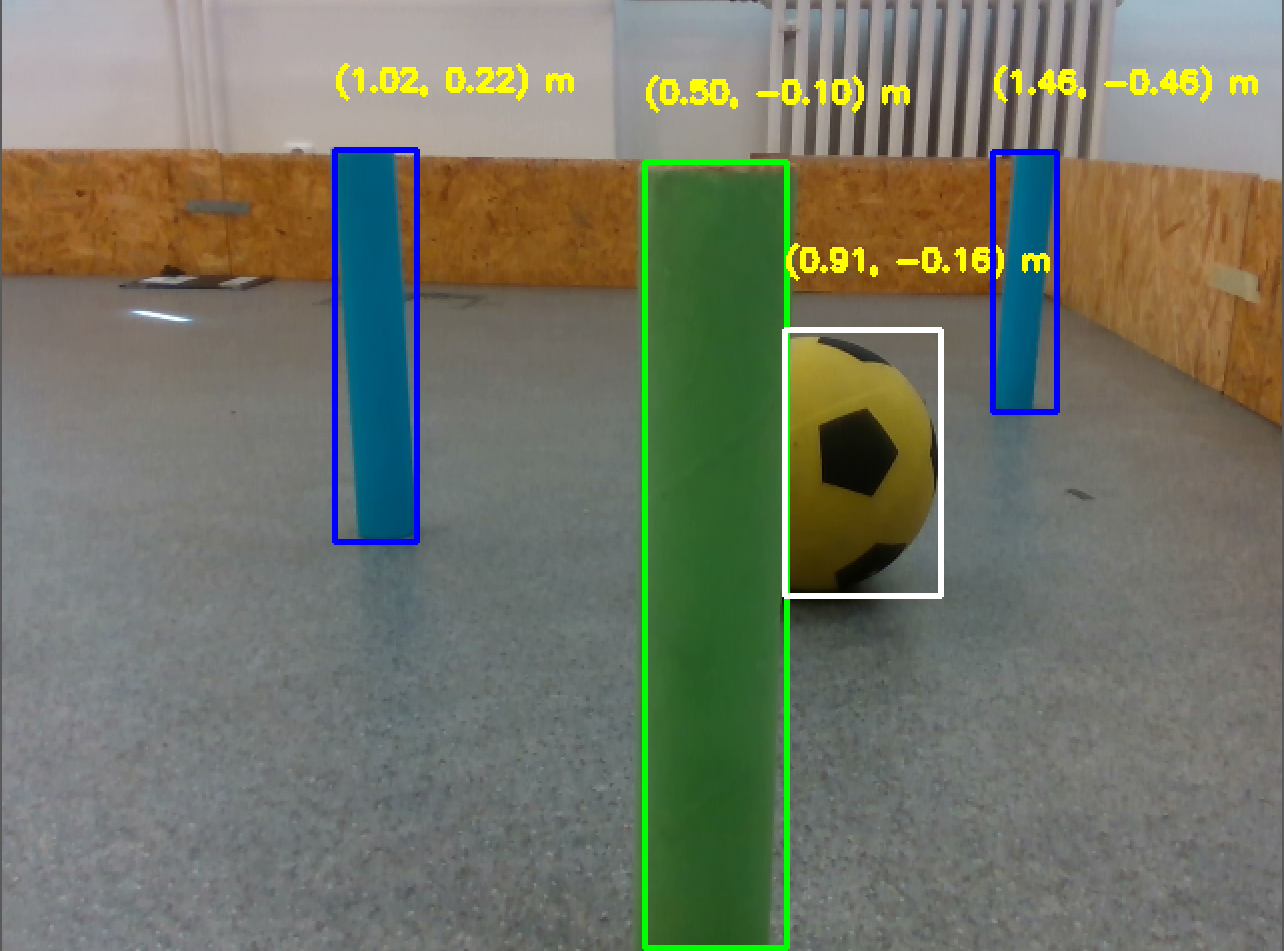
\includegraphics[width=0.5\textwidth]{pictures/detect.png}
    \caption{Obrázek z RGB kamery s rozpoznanými objekty}
    \label{fig:detect}
\end{figure}
\begin{figure}[H]
    \centering
    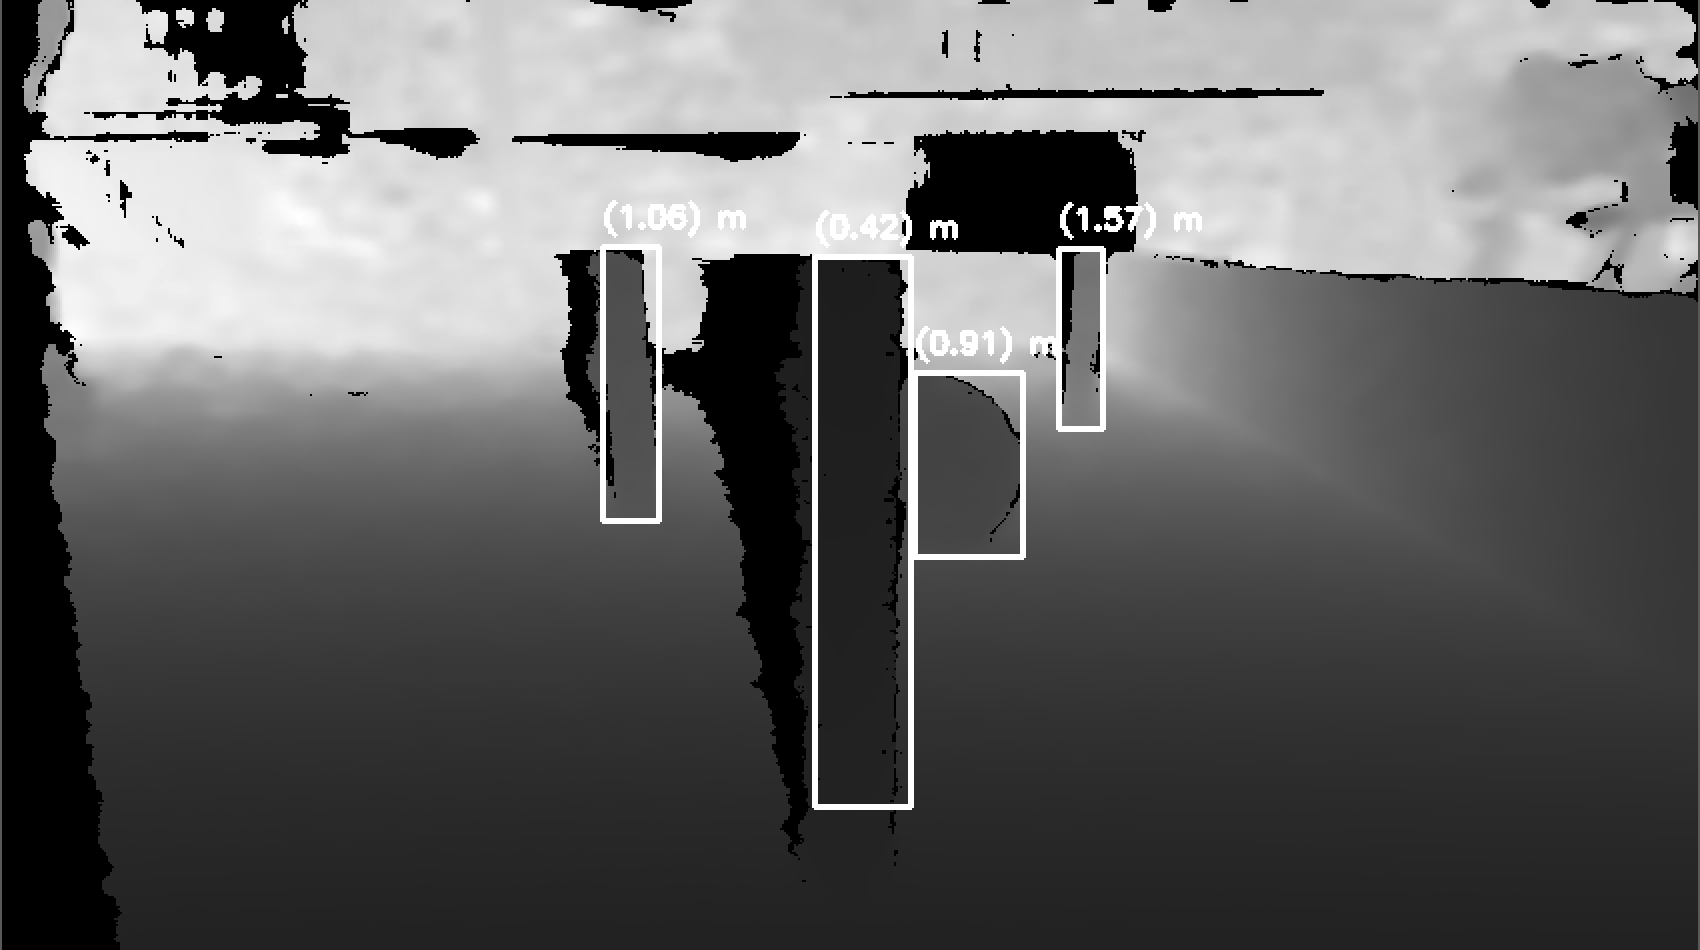
\includegraphics[width=0.7\textwidth]{pictures/depth_detect.png}
    \caption{Obrázek z hloubkové kamery s rozpoznanými objekty}
    \label{fig:depth_detect}
\end{figure}
Hloubková kamera vrací pouze pixeli s hloubkou. Aby byla poloha objektů spočítána co nejrychleji, pracujeme pouze s pixeli z hloubkové kamery (Obrázek \eqref{fig:depth_detect}), které jsou detekovány jako objekty z RGB kamery (Obrázek \eqref{fig:detect}).
Nejdříve vytvoříme transformační matici, která převadí mezi souřadnicemi kamery a hloubkové kamery. Poté se vypočítá median vzdáleností v bounding boxu, což řeší problém s obdelníky přesně nepasujícími na detekované objekty. 
Medián vzdálenosti přenásobíme konstantou 1.04, abychom korigovali nepřesnost depth kamery.
Pomocí K matice převedeme souřadnice z pixelů na reálné souřadnice vůči robotovi. Za souřadnice detekce se také přidá třída objektu.



\subsection{SLAM}
\subsection{Plánování}
\subsection{Pohyb}
\section{Závěr}




\end{document}